\chapter{弦微扰论}
\label{chap:4}
本节核心是将\ref{eq:2.39}的规范固定于黎曼曲面模空间相联系,并利用鬼场进行计算。弦微扰论目前前沿研究方向可见\cite{berkovits2022snowmasswhitepaperstring},超弦的规范固定比较复杂,详细可见\cite{Witten:2012bh}。本节还给出了一些玻色弦和超弦振幅的计算例子,以及Kawai-Lewellen-Tye关系\cite{Kawai:1985xq}和单值关系\cite{Bjerrum-Bohr:2009ulz}。

\section{模空间测度}
\ref{eq:2.39}的路径积分是对所有$\text{diff}\times\text{Weyl}$二维闭曲面等价类($\mathcal{D}g$)以及到靶空间的嵌入($\mathcal{D}X$)的求和。在数学上,$\text{diff}$的等价类由黎曼流形描述,多模去$\text{Weyl}$的等价类则由一维复流形,也就是黎曼曲面描述。我们首先从数学上对此进行叙述,这是代数几何中标准的内容\cite{forster2012lectures,schlichenmaier2010introduction,griffiths2014principles},我们选用更容易接受的物理些的讲法\cite{Giacchetto:2024aka,Staessens:2010vi}。
\subsection{黎曼曲面模空间}
黎曼曲面本身的定义是不含度规的,但是考虑在二维曲面$M$上加入不同的度规结构$[g]_{\text{diff}}$使之称为黎曼流形。下标$\text{diff}$提醒度量本身与坐标卡选取无关\footnote{在物理上微分同胚变换总是用不严谨的坐标变换替代,而数学上更偏向使用坐标无关的语言。}。可以证明任意一个度规结构$g$都给定了$M$上的复结构,而且此复结构仅仅依赖于度规的共形结构,也就是等价类$[g]_{\text{diff}\times\text{Weyl}}$,反过来,任意一个黎曼曲面都存在唯一一个与复结构相容的共形结构$[g]$。这样我们就把${\mathcal{D}[g]_{\text{diff}\times\text{Weyl}}}$的计算彻底与黎曼曲面上的复结构关联起来了。

类似微分同胚的定义,可以给出黎曼曲面之间全纯同构(共性等价)的概念,全纯同构对黎曼曲面进行了非常强的划分:

\begin{boxedtext}[单值化定理]
任何黎曼曲面$M$都共形等价于$\hat{M}/\pi_1(M)$,其中$\hat{M}$为$M$的泛覆叠空间,有下面几种情况:
\begin{equation*}
	\hat{M}=\left\{\begin{array}{c}\mathbb{C}\cup\{\infty\}\cong\mathbb{CP}^1\\\mathbb{C}\\\mathbb{H}\end{array}\right.
\end{equation*}
其中$\mathbb{H}$是上半复平面。
\end{boxedtext}

但是我们真正希望考虑的是复结构,复结构对黎曼曲面的刻画比全纯同构细的多。或者说不同的复结构之间可以是全纯同构的。而复结构的刻画就依赖于黎曼曲面的模空间,记为$\mathfrak{M}_g$,下标$g$表示亏格。而亏格为$g$的黎曼面上的所有度量结构记作$\mathcal{M}_g$。

上面的叙述似乎较为抽象,更加具体的方法是利用复结构与$[g]$的一一对应:
\begin{equation}
	\label{eq:4.1}
	\delta g_{ab}=\mathrm{diff}\oplus\mathrm{weyl}\oplus\mathrm{moduli}=-2(P_1\delta\sigma)_{ab}+(2\delta\omega-\nabla\cdot\delta\sigma)g_{ab}+\sum_{k=1}^{\dim\mathfrak{M}_g}\delta t^k\partial_{t^k}\hat{g}_{ab}
\end{equation}
这里利用了$n$阶对称无迹张量$v$到$n+1$阶对称无迹张量$u$的算符$P_n$:\footnote{这里$|b|$表示$b$不参与下标对称化。}
\begin{equation}
	(P_nv)_{a_1\cdots a_{n+1}}\equiv\nabla_{(a_1}v_{a_2\cdots a_{n+1})}-\frac{n}{n+1}g_{(a_1a_2}\nabla_{|b|}v_{a_3\cdots a_{n+1})}^b
\end{equation}
且此算符是唯一的,其共轭算符$P_n^T$定义为:
\begin{equation}
	(P_n^Tu)_{a_1\cdot\cdot\cdot a_n}\equiv-\nabla_bu^b{}_{a_1\cdot\cdot\cdot a_n}
\end{equation}
式\ref{eq:4.1}中$\mathrm{diff}\oplus\mathrm{weyl}$是规范冗余,是等价类$[g]$内部的映射,而$\mathrm{moduli}$则是黎曼面上不同的复结构,是等价类之间的变换,$t^k$用来标记不同复结构。计算$\mathcal{D}[g]$首先要选取一个规范固定$\hat{g}$,然后利用$\mathrm{diff}\oplus\mathrm{weyl}$规范变换积分掉整个等价类$[\hat{g}]$,与$V_{\mathrm{diff}\times\mathrm{weyl}}$抵消,然后在模空间上进行积分跑遍所有的等价类$[g]$。先取规范固定,然后积分掉规范自由度的过程,可以用图\ref{fig:3}表示。思想其实和Yang-Mills理论一样,但是弦论中选取一个规范固定无法用规范变换$\zeta$跑遍所有的$\mathcal{D}g$,所以还需要最后用模空间积分遍历。
\begin{figure}[htbp]
	\centering
	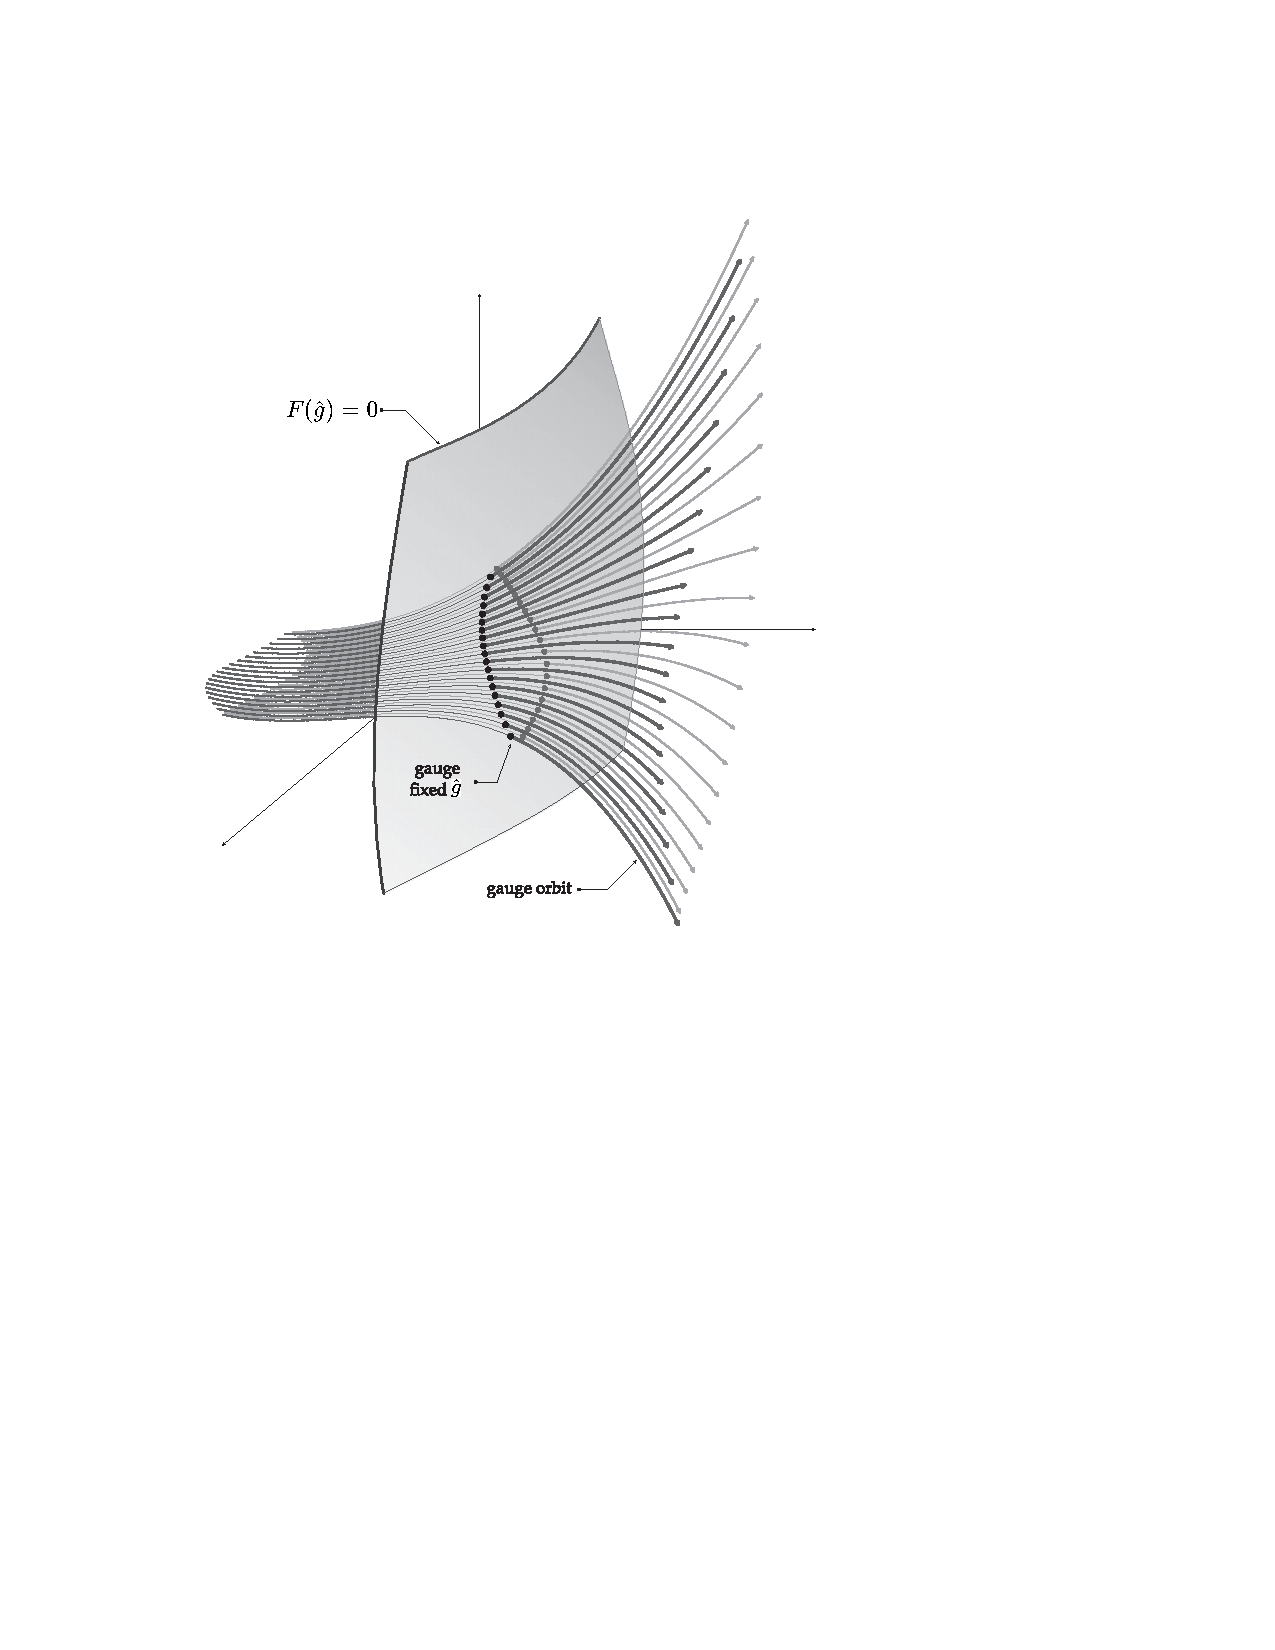
\includegraphics[width=0.5\linewidth]{figs/fig3.pdf}
	\caption{规范固定}
	\label{fig:3}
\end{figure}

虽然前面把$[g]$和复结构对应起来了,这告诉我们路径积分包含模空间的积分,但是为了对$\mathrm{diff}\oplus\mathrm{weyl}$积分,取规范固定$\hat{g}$后完全定下规范了吗?或者说我们建立了和规范变换$\zeta$和$[\hat g]$内元素的一一对应吗?这样$\int [\mathcal{D}\zeta]$才等于$V_{\mathrm{diff}\times\mathrm{weyl}}$从而完全消去规范冗余。但显然不是的,从前面光锥规范就能看出,单纯取等温坐标固定$g$没有完全定下规范,还又共形变换作为$\mathrm{diff}\oplus\mathrm{weyl}$的子群没有固定。同样的,规范变换$\zeta$跑遍了$[\hat g]$中的元素,但是$\mathrm{diff}\oplus\mathrm{weyl}$变换的子群CKG变换$\hat g$后仍得到$\hat g$,也就是说在规范固定点$\hat g$处仍有冗余的规范$V_{\mathrm{CKG}}$没有被消除。在数学上与之相关的群被称为黎曼曲面的自同胚群$\operatorname{Aut}(M)$。如果这个群是离散群,那么只需要除去$n_R=|\operatorname{Aut}(M)|$就可以消去规范,但是如果这个群是连续李群,这对应黎曼曲面$\pi_1(M)$是阿贝尔群的情况\footnote{对应的黎曼曲面称为例外黎曼面。},CKG的消去可以通过固定黎曼面上的某几个点来消去,也就是说规范选取变成了$(\hat g,\hat\sigma_{i\in\mathcal{F}})$,可以解释为固定了其中几个顶角算符的插入点\footnote{本文不考虑顶角算符个数不足以固定插入点的情况。},具体是固定哪几个顶角算符以及固定点的坐标$z_{i\in\mathcal{F}}$并不会影响最终的关联函数结果。自然联想到这种顶角算符的固定是通过积分顶角算符到无积分顶角算符之间的转换实现的,后面会看到的确如此。

上面规范固定的过程可以看作是下面的积分测度变换:
\begin{equation}
	\label{eq:4.4}
	\mathcal{D}gd^{2n}\sigma\to|J|\mathcal{D} \zeta d^{\mu}td^{2n-\kappa}\sigma
\end{equation}
其中$|J|$是变换的雅可比行列式。其中$\mu = \dim\mathfrak{M}_{g,n}$,$\kappa$则是CKG生成元个数。注意,在黎曼曲面上固定一个点需要一个“复”的CKG生成元,也就是一对实的CKG生成元来固定,例外是对于开弦顶角算符,由于其插入点在盘面边界圆周$\operatorname{Re}z=0$,所以只需要一个实的CKG生成元就能固定。后面谈到维数均指复维数。下面来计算几个简单黎曼面的自同胚群。

\begin{boxedtext}[黎曼曲面自同胚群]
	黎曼曲面$M$的自同胚群可以利用其基本群在其泛覆叠空间$\hat M$中的正规化子计算:
	\begin{equation*}
		\operatorname{Aut}(M)\cong N(\pi_1(M))/\pi_1(M),\quad N(G):=\{h\in \operatorname{Aut}(\hat{M})|hGh^{-1}=G\}
	\end{equation*}
\end{boxedtext}
所以首先要对三种不同的泛覆叠空间的自同胚群进行计算,结果如下:
\begin{equation}
	\operatorname{Aut}(\mathbb{CP}^1)\cong PSL(2,\mathbb{C}),\quad
	\operatorname{Aut}(\mathbb{C})\cong \operatorname{Aff}(1,\mathbb{C}),\quad
	\operatorname{Aut}(\mathbb{H})\cong PSL(2,\mathbb{R})
\end{equation}
注意到比如$\mathbb{CP}^1$和$\mathbb{H}$的自同胚群都包含两个连通分支,其中单位元存在的连通分支$\operatorname{Aut}_0(M)$才生成CKG。闭弦树级振幅涉及到球面,对应$\operatorname{Aut}_0(S^2)=SL(2,\mathbb{C})$,其有三个复自由度,所以可以固定球面上三个点。一圈振幅对应环面$\operatorname{Aut}_0(T^2)=\mathcal{T}_\mathbb{C}$,即由复平面上的平移群生成,所以可以在环面上固定一个点。同时离散对称性$\sigma^a\to -\sigma^a$同样不会改变环面上的$\hat{g}$,这个$\mathbb{Z}_2$对称性给出$n_R=2$。开弦树级振幅对应盘面也即上半复平面,对应CKG为$\operatorname{Aut}_0(D_2)\cong SL(2,\mathbb{R})$,有三个实自由度,所以同样可以固定盘面边界上三个顶角算符插入点。

模去共形Killing群后,我们考虑的黎曼曲面$\mathcal{M}_g$变成了带标记点的黎曼曲面$\mathcal{M}_{g,n}$,现在来关注其模空间$\mathfrak{M}_{g,n}$。注意到$\delta_m g_{ab}$与$\mathrm{diff\times weyl}$正交:
\begin{equation}
	\begin{aligned}
		0&=\int d^2\sigma g^{1/2}\delta_mg_{ab}\left[-2(P_1\delta\sigma)^{ab}+(2\delta\omega-\nabla\cdot\delta\sigma)g^{ab}\right]\\
		&=\int d^2\sigma g^{1/2}\left[-2(P_1^T\delta^{\prime}g)_a\delta\sigma^a+\delta_mg_{ab}g^{ab}(2\delta\omega-\nabla\cdot\delta\sigma)\right]\\
		&\Rightarrow  g^{ab}\delta_m g_{ab} =0,\quad (P^T_1\delta_m g)_a=0
	\end{aligned}
\end{equation}
第一个无迹条件自动满足,迹包含在Weyl变换项中,第二个条件说明模空间对应$\ker P^T_1$。另外CKG生成元满足的共形Killing方程可以写为:
\begin{equation}
	(P_1\delta\sigma)_{ab}=0
\end{equation}
所以CKG对应$\ker P_1$,模空间维数与CKG维数之间有如下公式:
\begin{boxedtext}[Riemann-Roch公式]
	\begin{equation}
		\label{eq:4.8}
		\dim\ker P_n-\dim\ker P_n^T=(n+\frac12)\chi=(2n+1)(1-g)
	\end{equation}
\end{boxedtext}
上式\ref{eq:4.8}只是Riemann-Roch定理的一个特例。注意到$\kappa$正好对应黎曼曲面上固定点的个数,所以上述结果可以推广到固定点任意多的黎曼曲面模空间:
\begin{boxedtext}[模空间维数]
	亏格为$g$且带$n$个标记点的黎曼曲面模空间是一个连通光滑的复轨形,维数为:
	\begin{equation}
		\label{eq:4.9}
		\dim\mathfrak{M}_{g,n} = 3 g - 3 + n
	\end{equation}
	且我们考虑$2g-2+n>0$情况,这对应$\operatorname{Aut}(M_{g,n})$是有限群,也即固定点后完全模去了CKG。
\end{boxedtext}
模空间是一个复轨形来源于其有如下的计算方式\footnote{考虑不带标记点的简单情况。}:
\begin{boxedtext}[Teichm\"uller空间]
	$\mathrm{Diff}^+$表示保定向的微分同胚变换,$\mathrm{Diff}_0$表示与单位映射同伦的微分同胚。则定义模群$\Gamma_g$\footnote{也常称为Mapping Class Group。}和Teichm\"uller空间$\mathfrak{T}_g$:
	\begin{equation*}
		\Gamma_\mathrm{g}:=\mathrm{Diff}^+(M)/\mathrm{Diff}_0(M),\quad \mathfrak{T}_\mathrm{g}\equiv\frac{\mathcal{M}_g}{\mathrm{Weyl}(M)\times\mathrm{Diff}_0(M)}
	\end{equation*}
	黎曼曲面模空间有如下轨形形式:
	\begin{equation}
		\label{eq:4.10}
		\mathfrak{M}_\mathrm{g}=\mathfrak{T}_\mathrm{g}/\Gamma_\mathrm{g}
	\end{equation}
\end{boxedtext}
利用\ref{eq:4.9}计算发现球面$g=0,n=3$情况模空间平凡,所以树图振幅不涉及模空间积分的计算。第一个非平凡的例子是环面$g=1,n=1$,模空间维数为$1$,环面上的复结构由下面的格生成:
\begin{equation}
	\Gamma:=\mathbb{Z}\alpha_1+\mathbb{Z}\alpha_2=\{n\alpha_1+m\alpha_2:n,m\in\mathbb{Z}\}
\end{equation}
$T^2 \cong  \mathbb{C}/\Gamma$,$\alpha_{1,2}\in\mathbb{C}$。不同复结构由$SL(2,\mathbb{Z})$意义下不同构的格生成。两个复自由度$\alpha_1,\alpha_2$约化为一个。在\ref{eq:4.10}的观点下,环面的模空间为:
\begin{equation}
	\mathfrak{M}_{1,1}=\mathbb{H}/PSL(2,\mathbb{Z})
\end{equation}
所以模空间参数$\tau$可以通过模群限制在图\ref{fig:5}所示的阴影部分中,即模空间积分范围为:
\begin{equation}
	\mathscr{F}:=\left\{\tau\in\mathscr{H}:-\frac{1}{2}\leq\mathrm{Re}(\tau)\leq\frac{1}{2},|\tau|\geq1\right\}
\end{equation}
这种模空间边界的自然存在性,或者说因为模不变性,让弦论自然拥有一个截断,从而是紫外有限的理论。\cite{Witten:2015mec}
\begin{figure}[htbp]
	\centering
	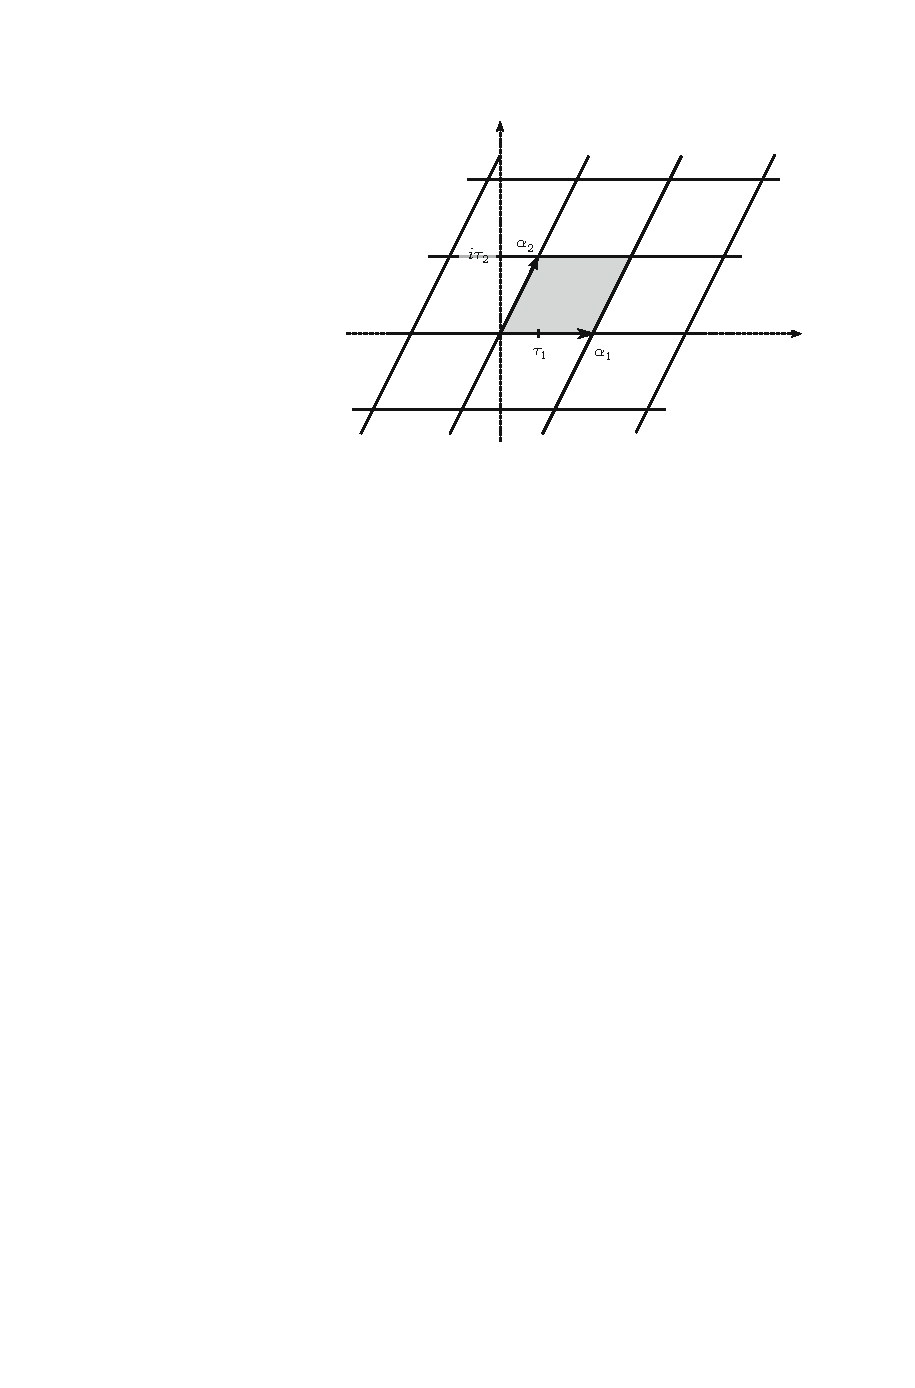
\includegraphics{figs/fig4.pdf}
	\caption{环面上不同的复结构,在$SL(2,\mathbb{Z})$同构的意义下,取$(\alpha_1,\alpha_2)=(1,\tau)$}
	\label{fig:4}
\end{figure}
\begin{figure}[htbp]
	\centering
	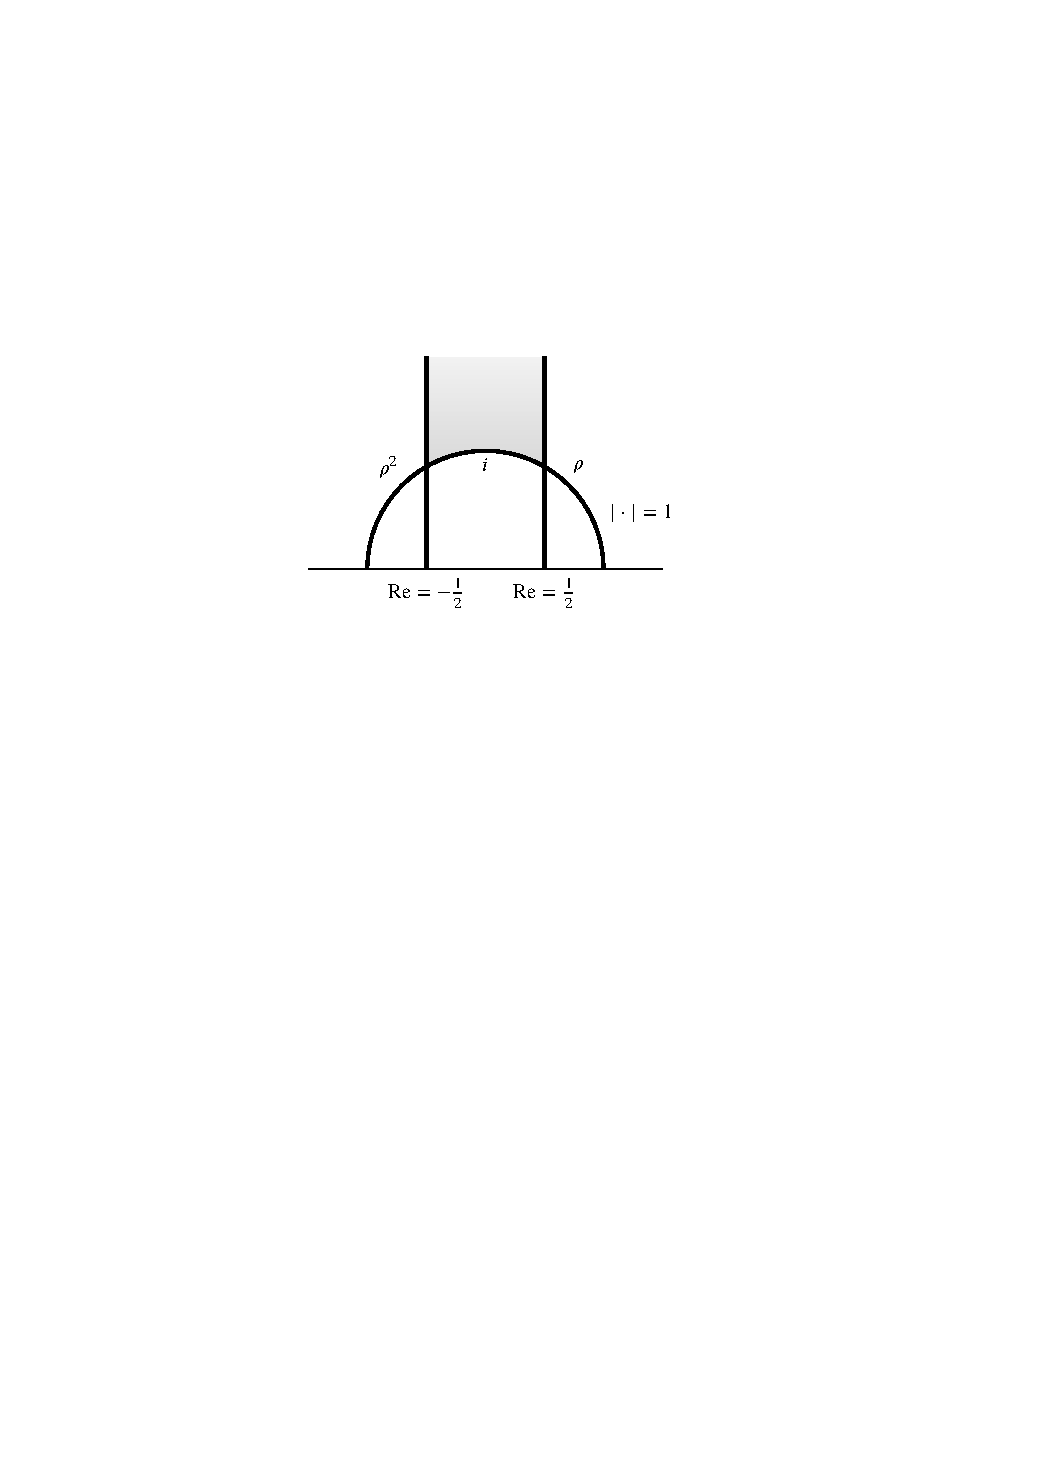
\includegraphics{figs/fig5.pdf}
	\caption{环面模空间的基本域,$\rho:=e^{2\pi i/6}$}
	\label{fig:5}
\end{figure}

在黎曼面上积分的想法近年来也从弦论渗透到了场论振幅计算中,Cachazo-He-Yuan形式给了场论振幅利用带标记点黎曼面上积分的统一形式\cite{Cachazo:2013iea,Cachazo:2013hca}:
\begin{equation}
	\mathcal{A}_{n}^\text{tree}=\int d\mu_{n}\mathcal{I}_{n}^L\mathcal{I}_{n}^R,\quad d\mu_{n}=\frac{d^{n}\sigma}{\mathrm{volSL}(2,\mathbb{C})}{\prod_{a}}^{\prime}\delta{\left(\sum_{b\neq a}\frac{s_{ab}}{\sigma_{ab}}\right)}
\end{equation}
不同场论的区别在于CHY被积函数$\mathcal{I}$,但是树级振幅都有上述的统一形式!
\subsection{FP量子化}
现在来计算\ref{eq:4.4}中的Jacobi行列式,这个积分测度变换对应插入:
\begin{equation}
	1=\Delta_{\mathrm{FP}}(g,\sigma)\int_\mathfrak{M}d^\mu t\int_\mathrm{diff\times Weyl}\mathcal{D}\zeta\delta(g-\hat{g}(t)^\zeta)\prod_{(a,i)\in \mathcal{F}}\delta(\sigma_i^a-\hat{\sigma}_i^{\zeta a})
\end{equation}
利用\ref{eq:4.1}以及标准的FP鬼场方法计算得到:
\begin{equation}
	\label{eq:4.16}
	\Delta_{\text{FP}}=\frac{1}{n_R}\int\mathcal{D}b_{ab}\mathcal{D}c^a\exp(-S_g)\prod_{k=1}^\mu\frac{1}{4\pi}(b,\partial_{t^k}\hat{g})\prod_{(a,i)\in \mathcal{F}}c^a(\hat{\sigma}_i),\quad S_g=\frac{1}{2\pi}\left(b,(\hat{P}_1c)\right)
\end{equation}
当$\hat g$取共形规范时$b_{ab}$和$c^a$退化为全纯和反全纯左右模,也即\ref{eq:2.32}形式。这里涉及到对称无迹张量之间的内积,定义为:
\begin{equation}
	\label{eq:4.17}
	(t,t^\prime)_{\hat g}:=\int d\sigma^a {\hat g}^{\frac{1}{2}} (t\cdot t^\prime)
\end{equation}
这里$\cdot$表示对所有指标缩并。\ref{eq:2.39}规范固定后的形式为:
\begin{equation}
	\label{eq:4.18}
	\begin{aligned}
		S_{j_1...j_n}(k_1,\ldots,&k_n)=\sum_{\substack{\text{worldsheet}\\\text{topologies}}}\int_{\mathfrak{M}}\frac{d^\mu t}{n_R}\mathcal{D}X\mathcal{D}b\mathcal{D}c\exp(-S_\mathrm{m}-S_\mathrm{g}-\lambda\chi)\\&\times\prod_{(a,i)\notin \mathcal{F}}\int d\sigma_i^a\prod_{k=1}^\mu\frac{1}{4\pi}(b,\partial_{t^k}\hat{g})\prod_{(a,i)\in\mathcal{F}}c^a(\hat{\sigma}_i)\prod_{i=1}^n\hat{g}(\sigma_i)^{1/2}U_{j_i}(k_i,\sigma_i)
	\end{aligned}
\end{equation}
由此可见固定顶角算符插入点确实相当于将无积分顶角算符换为积分顶角算符。现在对$bc$进行模展开,将上式与$bc$鬼场零模的插入联系起来。
\begin{equation}
	\begin{gathered}
		c^a(\sigma)=\sum_Jc_J\mathsf{C}_J^a(\sigma),\quad b_{ab}(\sigma)=\sum_Kb_K\mathsf{B}_{Kab}(\sigma)\\
		P_1^TP_1\mathsf{C}_J^a=\mu_J^{2}\mathsf{C}_J^a,\quad P_1P_1^T\mathsf{B}_{Kab}=\nu_K^2\mathsf{B}_{Kab}
	\end{gathered}
\end{equation}
$\mathsf{C}_J$,$\mathsf{B}_{K}$在\ref{eq:4.17}内积的意义下正交归一。而且两者的非零模之间有一一对应:
\begin{equation}
	\mathsf{B}_{Jab}=\frac{1}{\nu_J}(P_1\mathsf{C}_J)_{ab},\quad\nu_J=\mu_J\neq0
\end{equation}
而且零模正好是$\ker P_1^T$和$\ker{P_1}$中的向量。FP行列式\ref{eq:4.16}路径积分可以直接用模展开得到:
\begin{equation}
	\label{eq:4.21}
	\begin{aligned}
		\Delta_{\text{FP}}=&\int\prod_{k=1}^\mu db_{0k}\prod_{j=1}^\kappa dc_{0j}\prod_Jdb_Jdc_J\exp\left(-\frac{\nu_Jb_Jc_J}{2\pi}\right)\prod_{m=1}^\mu\frac{1}{4\pi}(b,\partial_{t^{m}}\hat{g})\prod_{(a,i)\in\mathcal{F}}c^a(\sigma_i)\\
		=&\int\prod_{k=1}^\mu db_{0k}\prod_{m=1}^\mu\left[\sum_{k^{\prime}=1}^\mu\frac{b_{0k^{\prime}}}{4\pi}\left(\mathrm{B}_{0k^{\prime\prime}},\partial_{t^m}\hat{g}\right)\right]
		\int\prod_{j=1}^\kappa dc_{0j}\prod_{(a,i)\in\mathcal{F}}\left[\sum_{j^{\prime}=1}^\kappa c_{0j^{\prime}}\mathsf{C}_{0j^{\prime}}^a(\sigma_i)\right]
		\\
		&\times\int\prod_Jdb_Jdc_J\exp\left(-\frac{\nu_Jb_Jc_J}{2\pi}\right)\\
		=&\det\frac{(\mathsf{B}_{0k},\partial_{t^m}\hat{g})}{4\pi}{\det}\mathsf{C}_{0j}^a(\sigma_i){\det}^{\prime}\left(\frac{P_1^TP_1}{4\pi^2}\right)^{1/2}
	\end{aligned}
\end{equation}
第二个等号利用了格拉斯曼变量积分的性质,只有在被积函数为积分变量的最高形式时才不为零。最后一个等号中${\det}^\prime$表示不考虑零模贡献,否则显然$\det=0$。由上式不难看出规范固定的过程正是插入$bc$鬼场零模,而Riemann-Sroch定理$\mu-\kappa$给出的正是鬼数补偿,其正好补偿背景鬼数\ref{eq:2.66}。

虽然鬼场方法是极具物理思想的方法,但是其推导出来的结果右有非常清晰的物理解释。\ref{eq:4.21}中第三项可以看作是一个归一化系数不用过多考虑,第二项$c$鬼场零模正好对应CKG生成元,第一项在数学上相当于插入一些Beltrami微分,是复结构的体现。而且,单纯从形式上来说\ref{eq:4.18}有下面更简单的形式:

注意我们将所有的顶角算符插入点全部固定,而增加了Beltrami微分,这也是鬼数补偿的要求。相当于考虑亏格相同,但是固定点更多的模空间:
\begin{equation}
	\mathfrak{M}_{g,n+n_c+n_o},\quad \dim\mathfrak{M} = -\frac32 \chi + \frac12 n_o+n_c
\end{equation}
固定点的信息被转移到了模空间中去。但是从计算的角度上看依旧是\ref{eq:4.18}更方便,因为模空间积分计算比较复杂。

前面都是对玻色弦考虑的,超弦的情况要复杂得多。对于本篇论文,只要知道树图是平凡的,我们只需要关注物质场关联函数计算以及$c$鬼场的插入即可。RNS超弦唯一多要求绘景数求和为$2$。
\section{树级关联函数计算}
本节计算树级物质场和鬼场的关联函数,直接从路径积分出发计算,并说明此结果于OPE计算得到的结果相同。这里我们只对玻色部分物质场进行计算,本章最后计算超弦振幅时会直接使用OPE计算费米部分关联函数。



不难发现上面直接从路径积分得到的结果正好是OPE给出的关联函数奇异部分,实际上这并不是巧合,在树图层面上亚纯函数就是只依赖于奇异性。在后面处理纯旋量超弦的关联函数时会较多使用OPE方法。

\ref{eq:4.21}就是在算剩下的鬼场关联函数,涉及到的就是零模积分。OPE对应零模计算,物质场零模没有,剩下的鬼场零模要额外计算。
\section{玻色弦振幅}
稍微详细讲一下盘面振幅固定三个点之后注意顺序
\section{弦振幅之间的关系}
\subsection{KLT关系}
\subsection{单值关系}

\section{RNS超弦振幅}
